\chapter{Time-domain measurement of spin-torque switching in MTJs}

As we have discussed in the previous chapter, magnetization switchin induced by spin-tranfer torque is both useful for understanding the fundamental physics of magnetic dynamics and for applications in magnetic random access memory(MRAM). Measurements in the time domain can provide the most direct information about the switching process. However, the majority of previous time-resolved studies of spin-torque switching required averaging over many events, which would hide individual switching variations. Here we report a single-shot time resolved time-domain measurement similar to the technique developed by Cui.et.al \cite{Cui}. We have shown that the sensitivity of single-shot resistant measurements have been greatly improved and both prior to switching and during spin-torque switching have been resolved. 

\section{Experimental Setup}
Previously, the sketch of time-domain measurement is shown\ref{fig:time_set}. The general idea is the following: by send the pulse into the magnetic tunnel junctions, the transmitted the signal will depend on the resistance of the device. 

\begin{figure}[h]
  \centering
  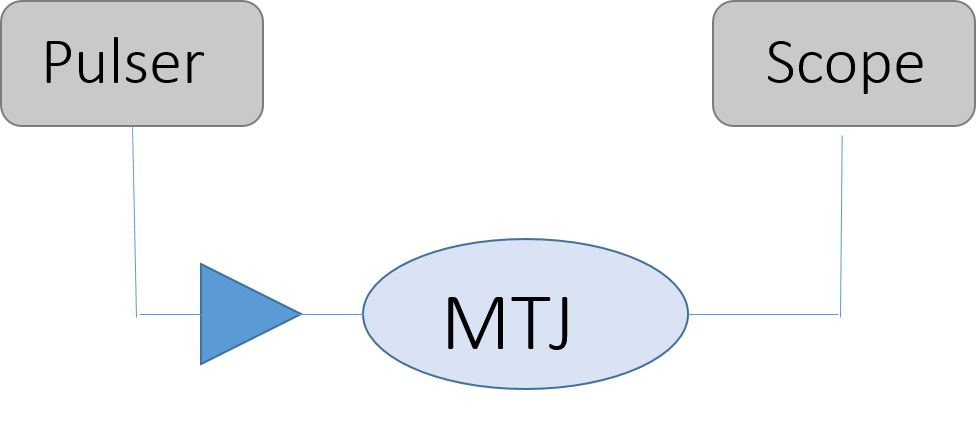
\includegraphics[width=0.6\textwidth]{fig/time_set.png}
  \caption{Original time-domain setup}
  \label{fig:time_set}
\end{figure}

If there is magnetic state switching happening during the duration of this pulse, we could be able to resolve it by recording the time-domain signal using a Time scope. This method is very straightforward, however, it is not practical in most cases. To illustrate that, let us calculate the transmitted signal.
 If we apply the voltage pulse$V_{inc}$, the transmitted signal will be given as

\begin{equation}
\label{orgi}
V(t) = \frac{V_{inc}}{1+G_S(t)Z_0/2}
\end{equation}
where $G_S(t) = 1/ R_S(T)$ is the sample conductance(the reciprocal resistance), $Z_0=50 \Omega$ is the probe impedance. Typically the resistance of the devices is around several thousands ohms, so we have a very strong impedance mismatching here. We can expand the time-dependent voltage signal with respect to a reference, if we use the parallel state conductance $G_P$ as the reference value, and write $G_S(t)$ as $G_S(t) = G_P + \Delta G(t)$, since $\Delta G(t) Z_0$ is usually much less than 1, we can expand Equation \ref{orgi} as the following:
\begin{equation}
\label{deltaequ}
V(t) = \frac{1}{1+G_PZ_0/2}V_{inc} + \frac{Z_0/2}{(1+G_PZ_0/2)^2}V_{inc} \Delta G(t)
\end{equation}

The first term in Equation\ref{deltaequ} is related to the resistance mismatch between the device and RF probe. The second term is coming from the resistance change associated with magnetic dynamics. If we would like to monitor the device resistance, we should expect the second term to be large, at least well above the noise level. However, as we point out, because of the impedance mismatching, the second term would be really smaller, usually around several mill volts. This requires lots of averaging to improve the signal to noise ratio and thereby hide each single switching event.

To improve our signal to noise ratio, we adapt improved measurement set-up shown in Fig.\ref{fig:time_domain}. As usual, we apply the pulse from a pulse generator. This time, however, we split the into two identical copies. The first copy goes into the device and induce magnetic switching. The second pulse will go through a pulse inverter and it will flip the polarity. What is important here is to choose the pulse inverter so that it does not distort the waveform too much. After the first copy goes through the device, we use a power combiner to combine these two pulses in a way that these two copies should enter the power combiner at the same time. 

\begin{figure}[h]
  \centering
  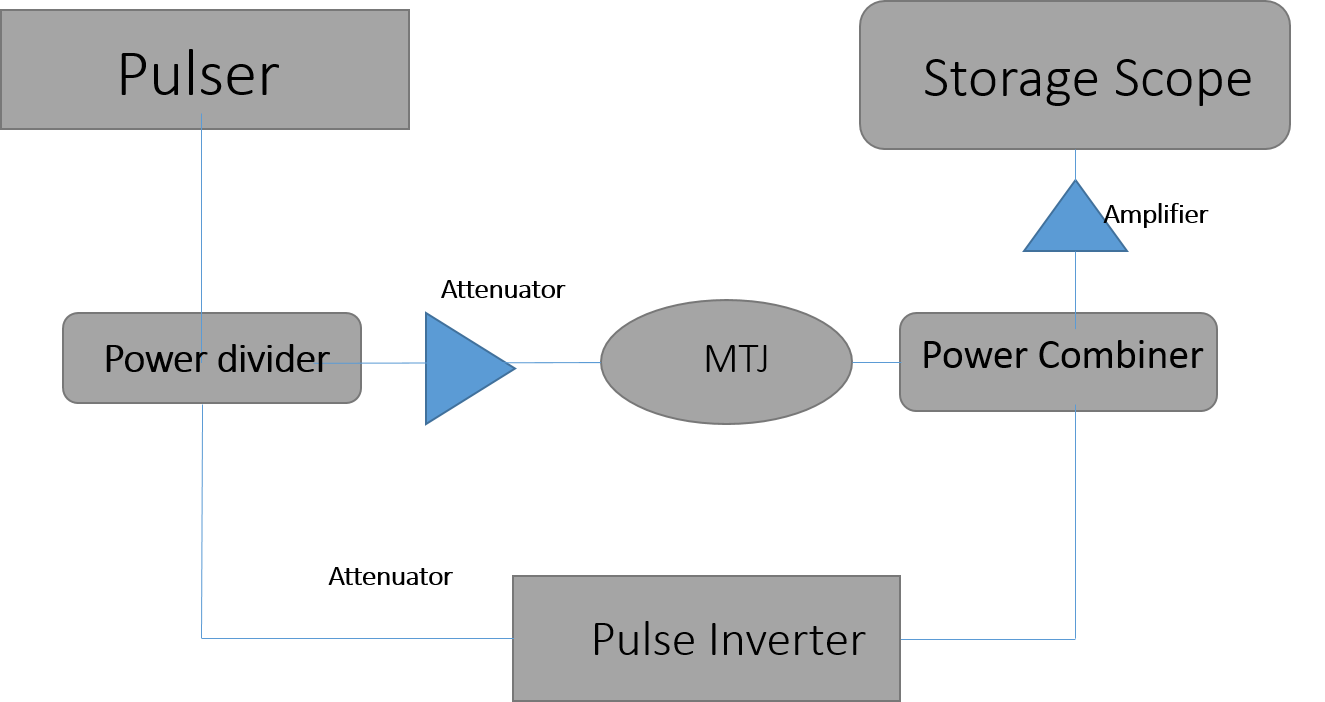
\includegraphics[width=0.8\textwidth]{fig/time_domain}
  \caption{Improve time-domain set-up}
  \label{fig:time_domain}
\end{figure}

To accomplish that, we would like to carefully tune the time delay of there two lines so that they have been correctly synchronized. In the current set-up, we adjust the time delay by varying the microwave cable length in the circuit. After we combine these two pulses, we use an amplifier to amplify the signal and send it into the storage scope. In this process, the signal left after we combine these two pulses would only be the part depending on the magnetic state, where any other type of noise should be canceled out. This should greatly improve the signal-to-noise ratio.

Before we go to the experiment discussion, we would like to discuss another important source of noises in these type of experiments. Ideally, we want to amplify our voltage signal after the power combiner to be large enough. However, we also have to fight with the bit noise induced by the storage scope. We are using a 64-bit time scope, the bit noise in the measurement is proportional to the voltage resolution used in the time scope. So in order to reduce the bit noise, smaller voltage resolution should be adapted and the signal has to be small enough to fit in this small voltage resolution. Practically, after we amplify the voltage signal, we use proper attenuator(usually around -10 dB).

\section{Results and Discussion}

Now we have set-up correct time delay and pick appropriate attenuation in the circuit, we can send the pulse and observe the time dependent signal. Fig.\ref{fig:Total_sig} shows a typical signal we resolve from a switching. We first initialize the MTJ into anti-parallel state and send through a positive pulse. The polarity of positive pulse corresponds to damping for the anti-parallel state, so this positive pulse should not induce magnetic switching for anti-parallel state. We record the anti-parallel state signal as the background and label it as AP in Fig.\ref{fig:Total_sig}. 

\begin{figure}[h]
  \centering
  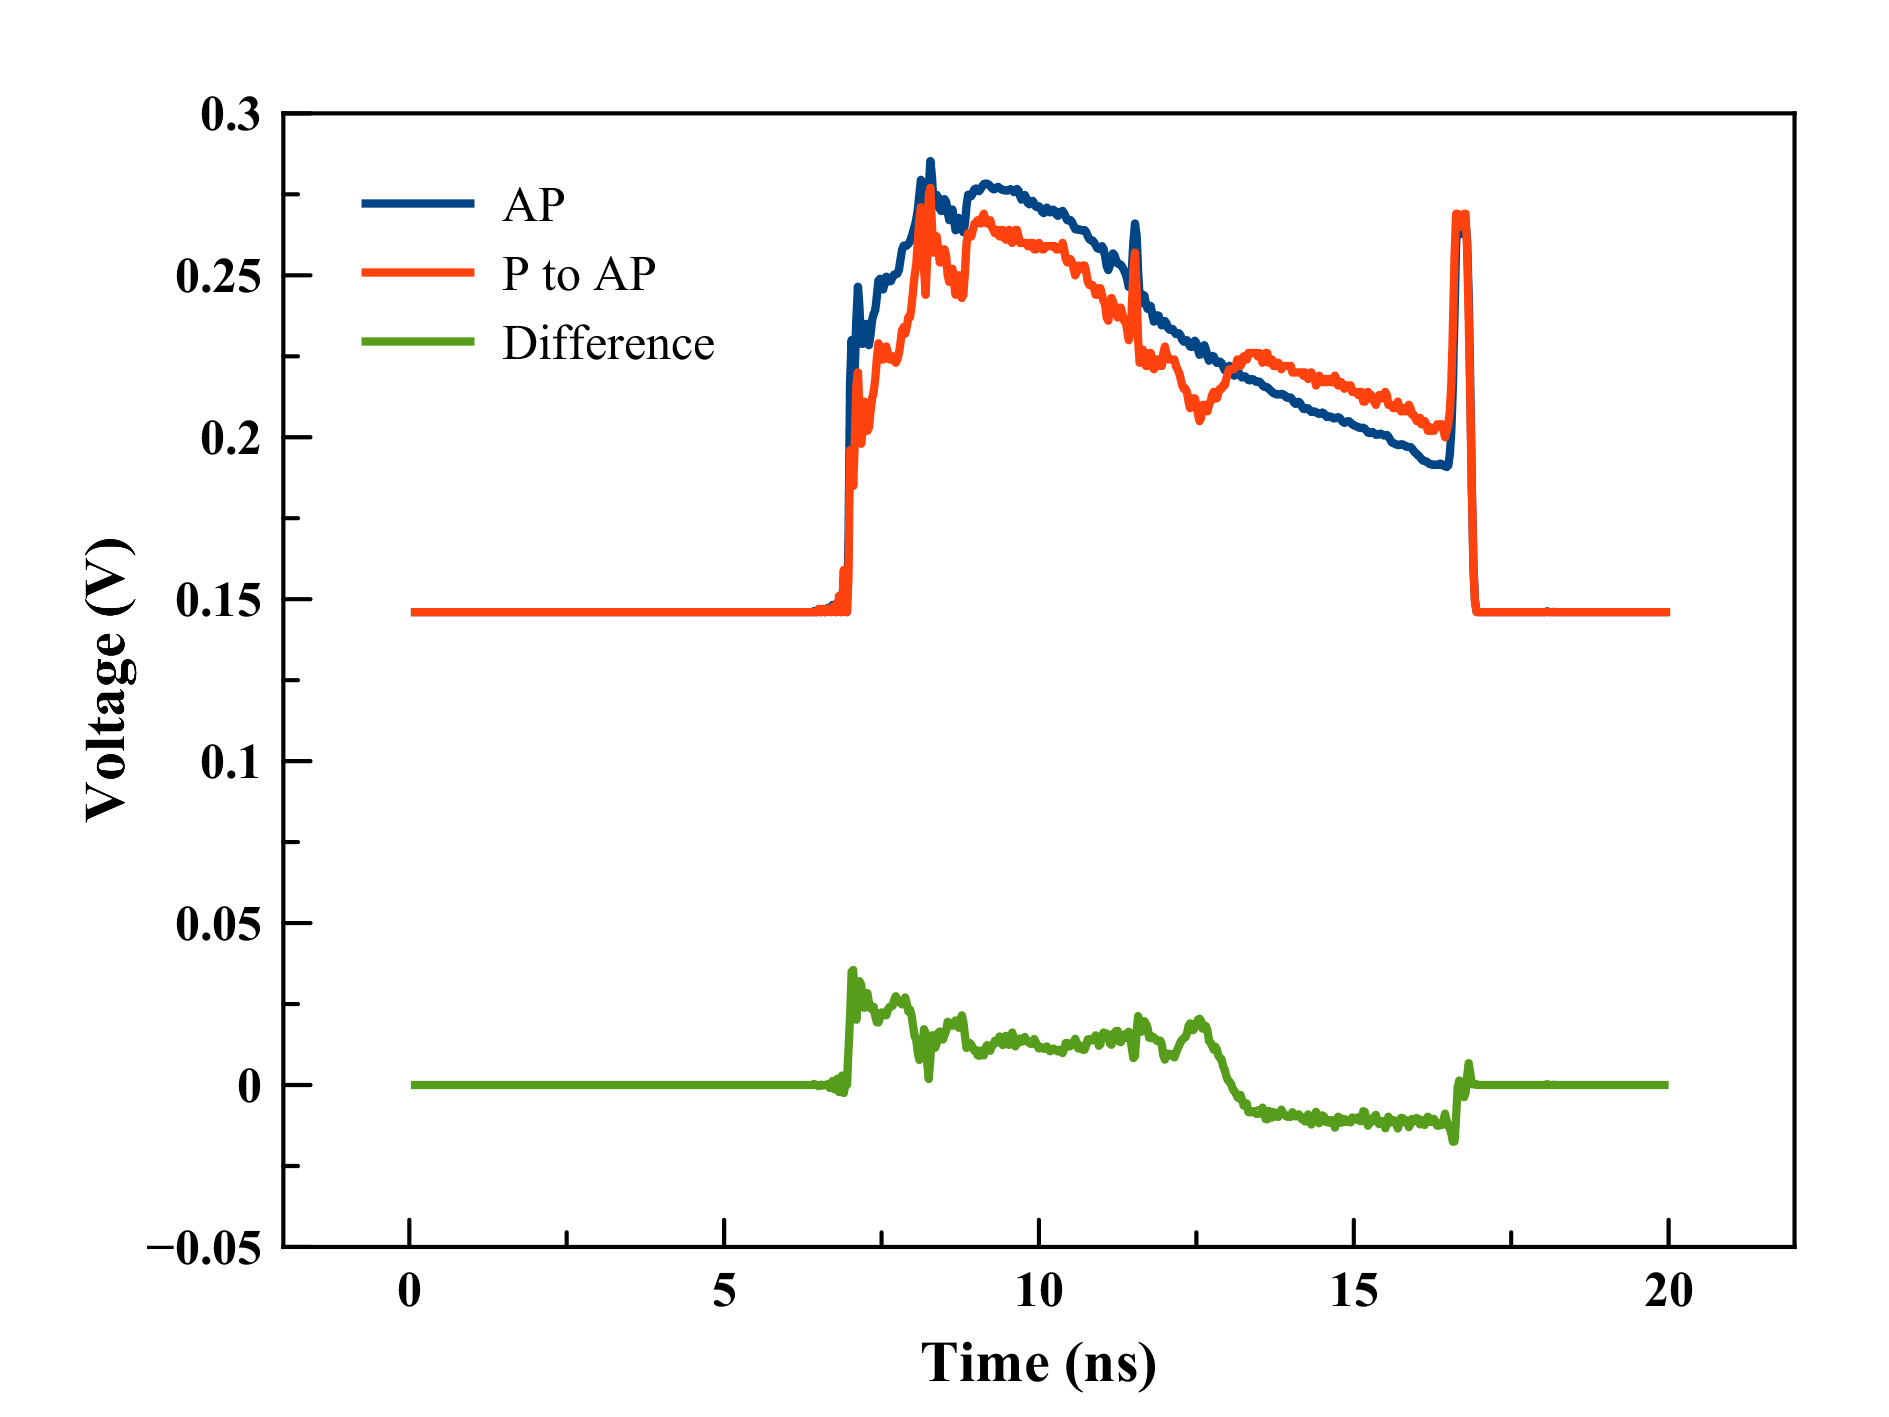
\includegraphics[width=0.8\textwidth]{fig/total_sig}
  \caption{A switching signal from time-domain measurement. Anti-parallel signal(blue), PtoAP signal(red) along with the voltage difference(Green)}
  \label{fig:Total_sig}
\end{figure}


Then, we initialize the MTJ into parallel state and re-send the positive voltage(which is anti-damping for parallel state). Then we record this signal from the time scope and label as P to AP in Fig.\ref{fig:APtoP}. One can clearly find that at the beginning of the pulse, AP and PtoAP signal are clearly separated. At the middle of the pulse, the PtoAP pulse suddenly shifts into AP signal, which is related to the magnetic state change in the MTJ. So we have observe a magnetic switching in time-domain. We can also subtract the background AP signal from the PtoAP and plot it labeled as Difference in Fig.\ref{fig:diff}. If we look at the Difference signal, we can see that at the beginning of the pulse, the difference is around 30 mV, then it drops to - 10 mV. So we can well separate the anti-parallel and parallel state.

\begin{figure}[!ht]
\centering
\subfigure{\label{fig:APtoP}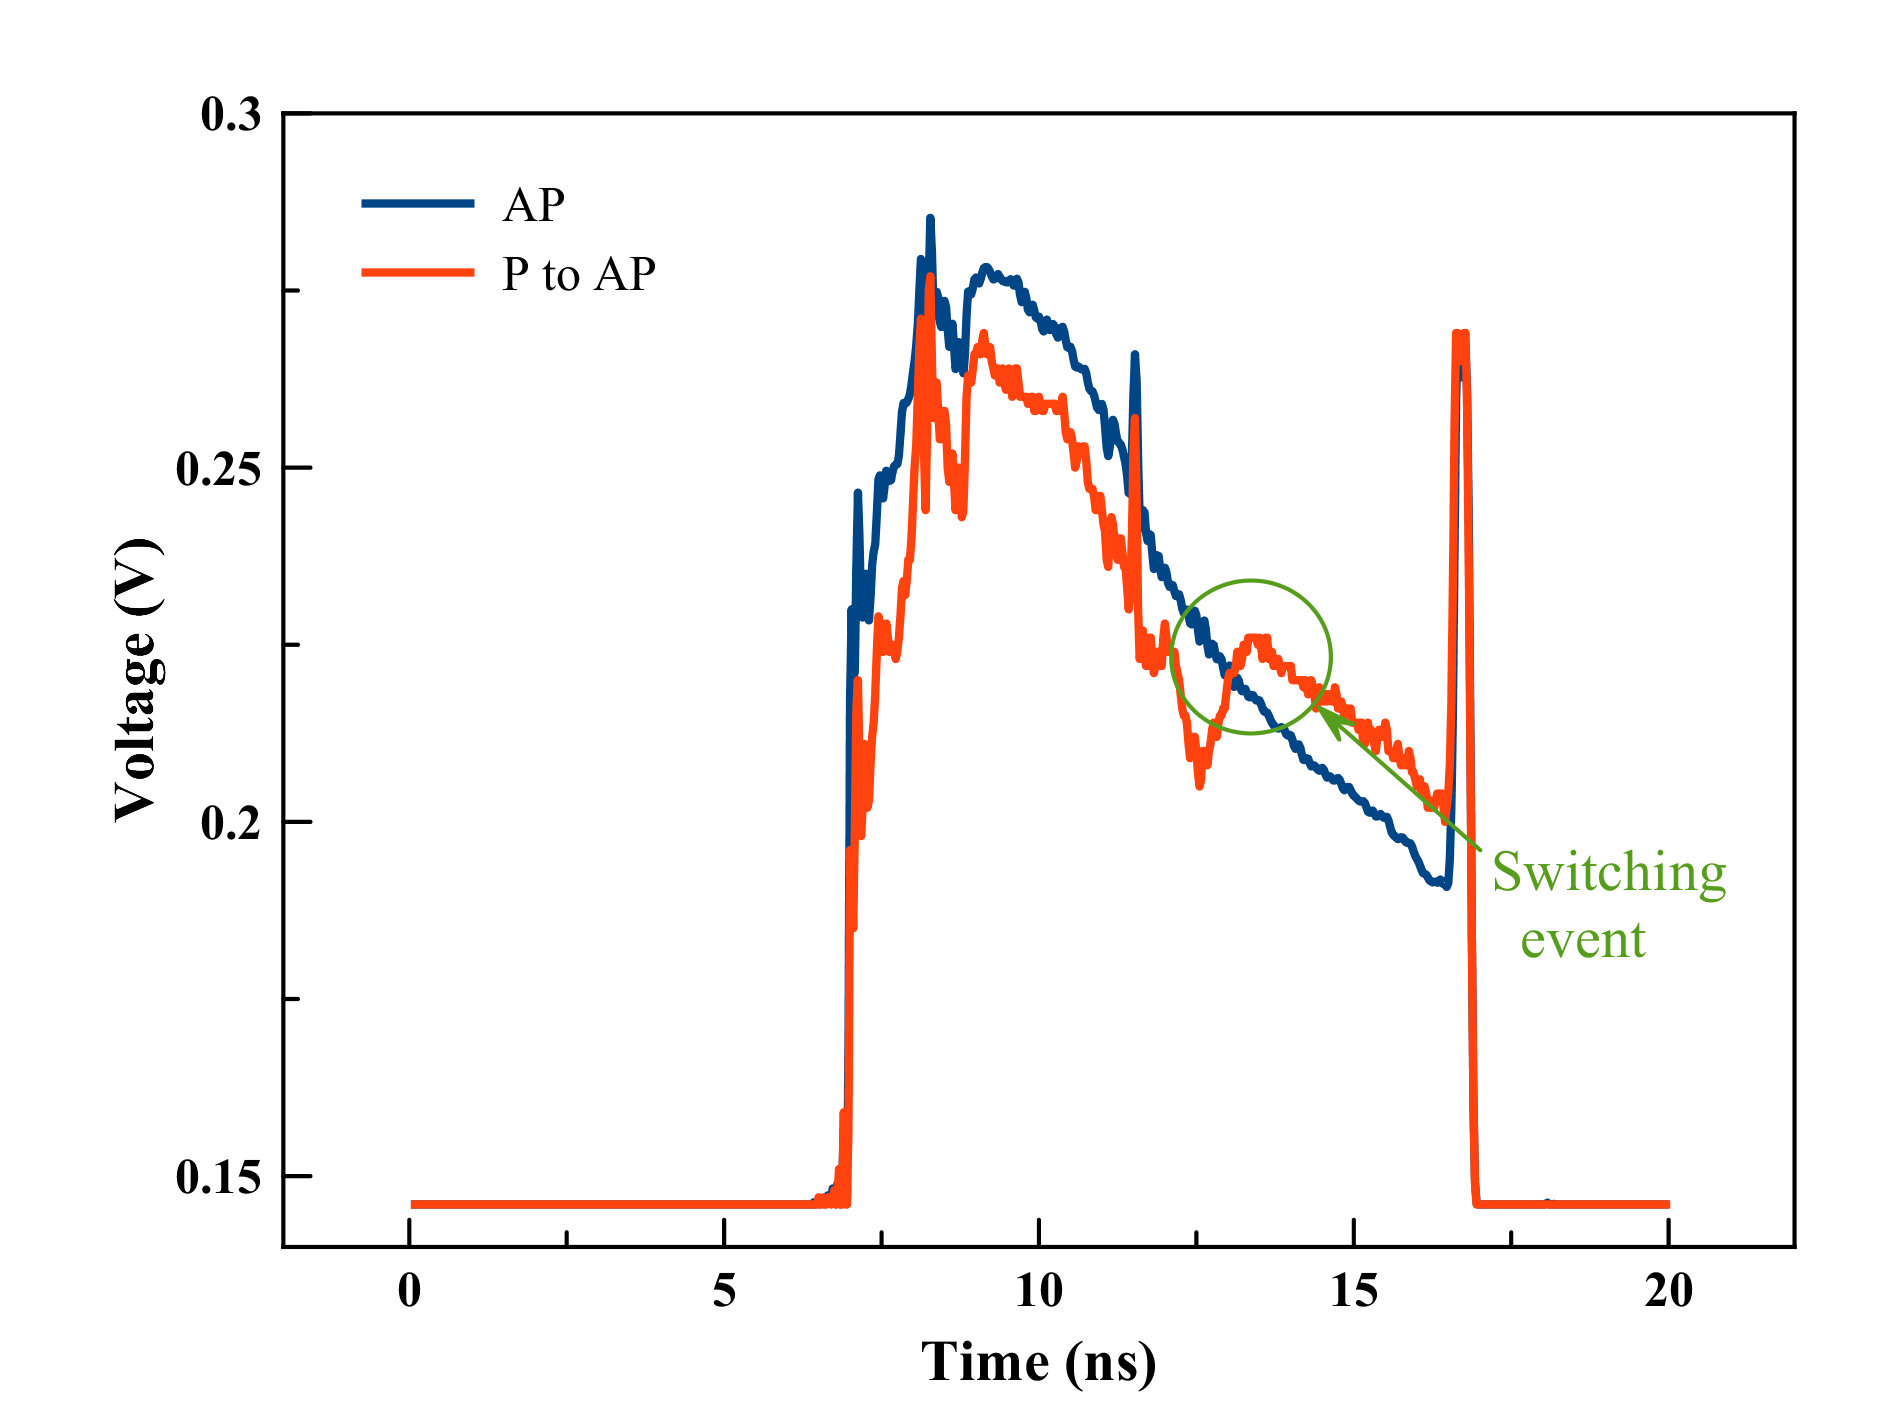
\includegraphics[width=80mm]{fig/APtoP.png}}
\subfigure{\label{fig:diff}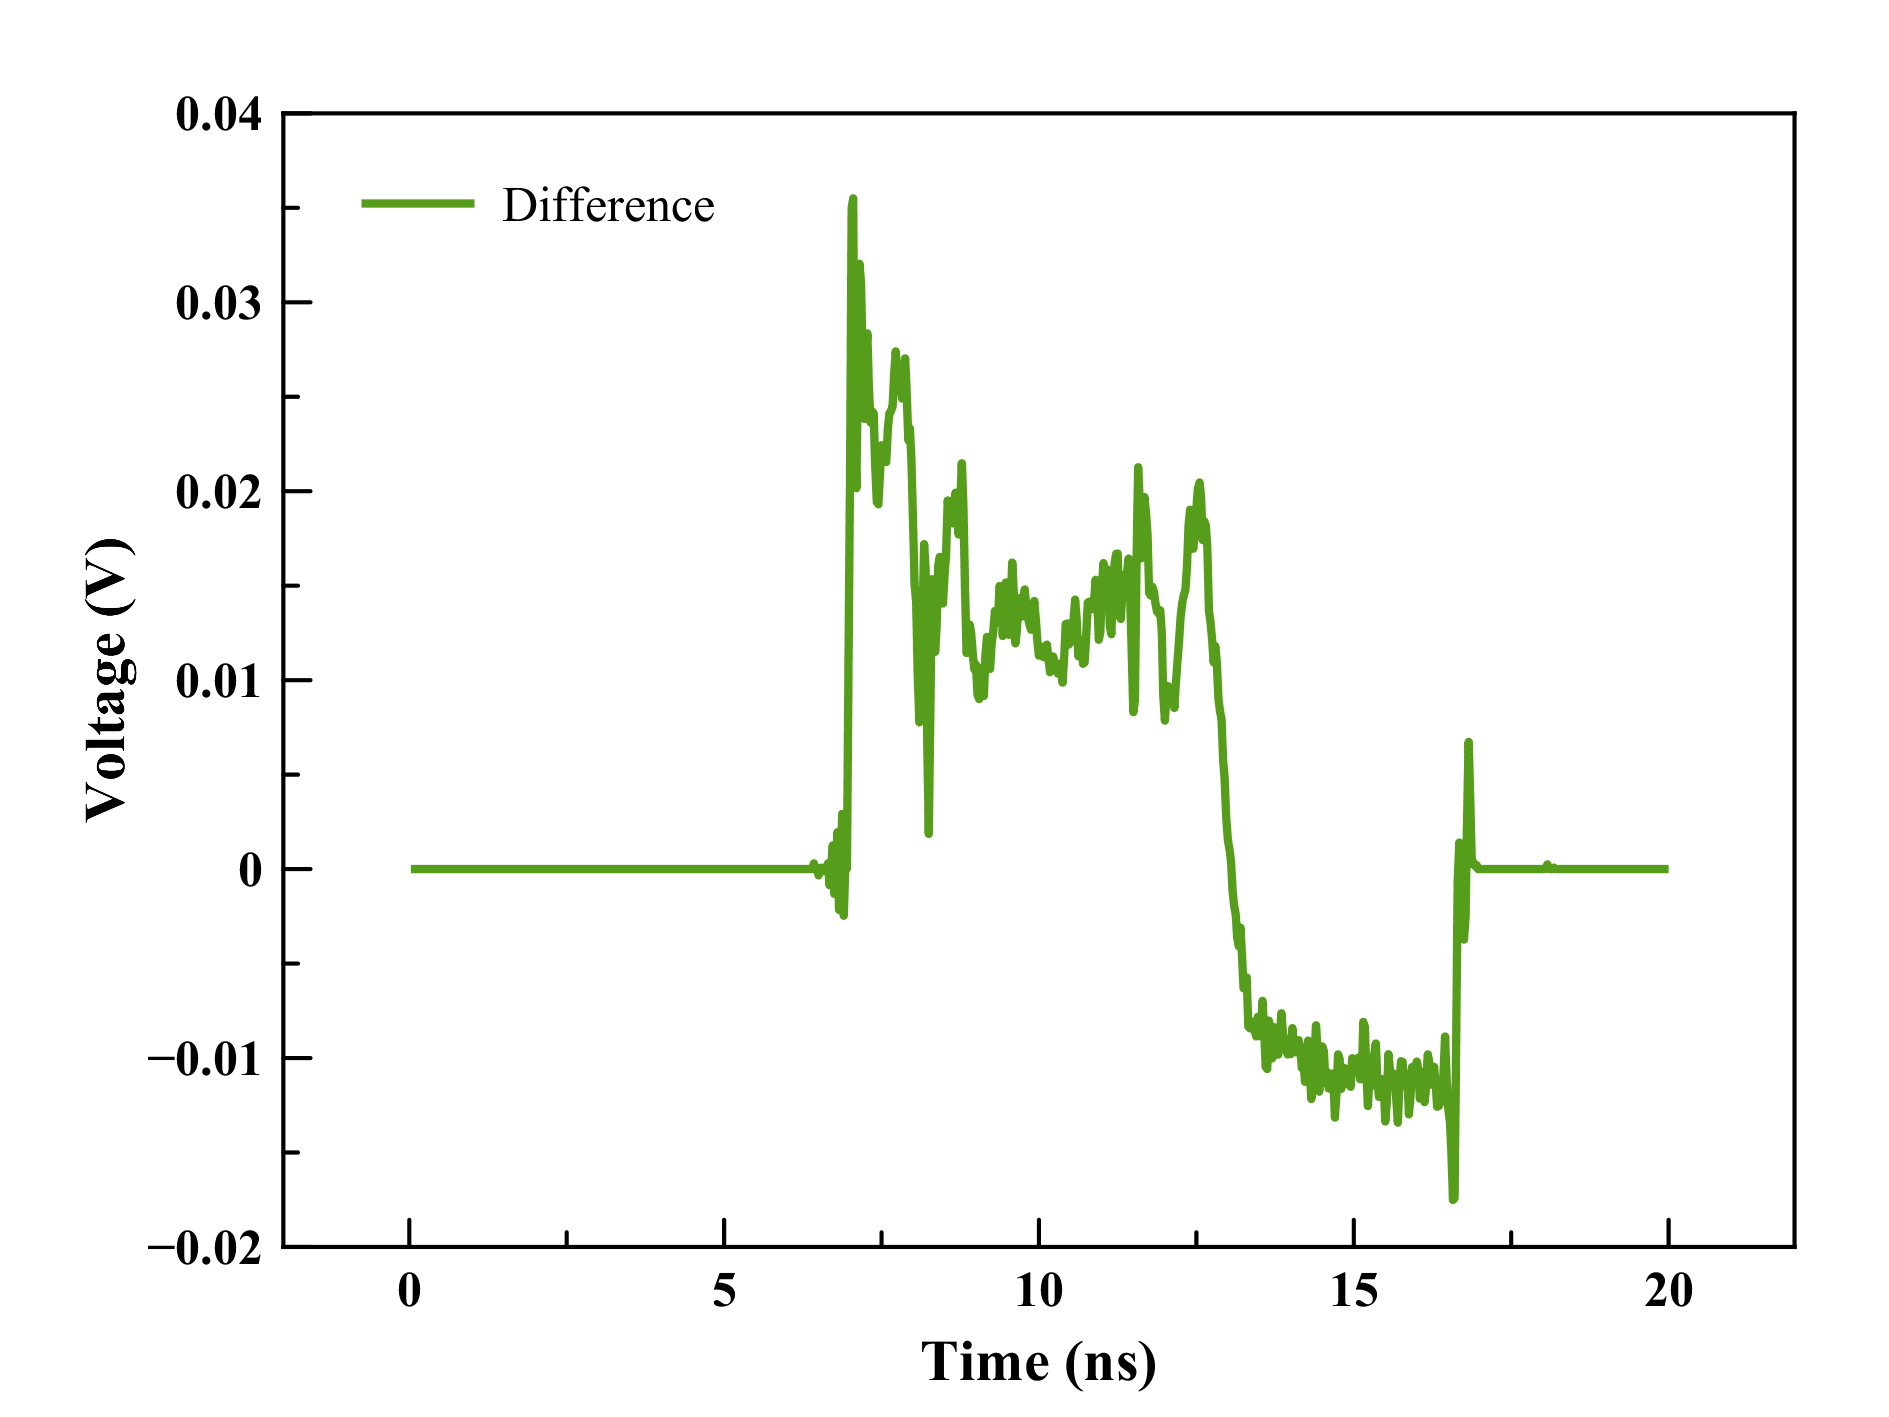
\includegraphics[width=80mm]{fig/diff.png}}
\caption{(a) Zoomed PtoAP signal(red) and AP state background(blue) (b)Zoomed voltage signal difference.}
\end{figure}

Now that we have greatly improved the voltage signal to separate two magnetic states, we can study individual switching event without perform averaging to reduce the noise. One thing we can study is the distribution of switching time. From Fig.\ref{fig:26} to Fig.\ref{fig:9} we show several traces from different switching events. Here we only demonstrate the different signals between two state. One can clear find that for different switching traces, we have different switching time, ranging from 2.6 ns, which is at the beginning of the pulse, to 9 ns, which is at the very end of the pulse. This indicates the random nature of this single shot-switching. More importantly, we can obtain a good statistics of switching time as a function of input parameters. Also we find that in Fig.\ref{fig:no} we find that at a fixed voltage, we can still have non-successful switching event, where we find that for this non-successful switching attempt, the system enters a large oscillation. This enables us to further study the different between successful and non-successful switching events. 




\begin{figure}[!ht]
\centering
\subfigure{\label{fig:26}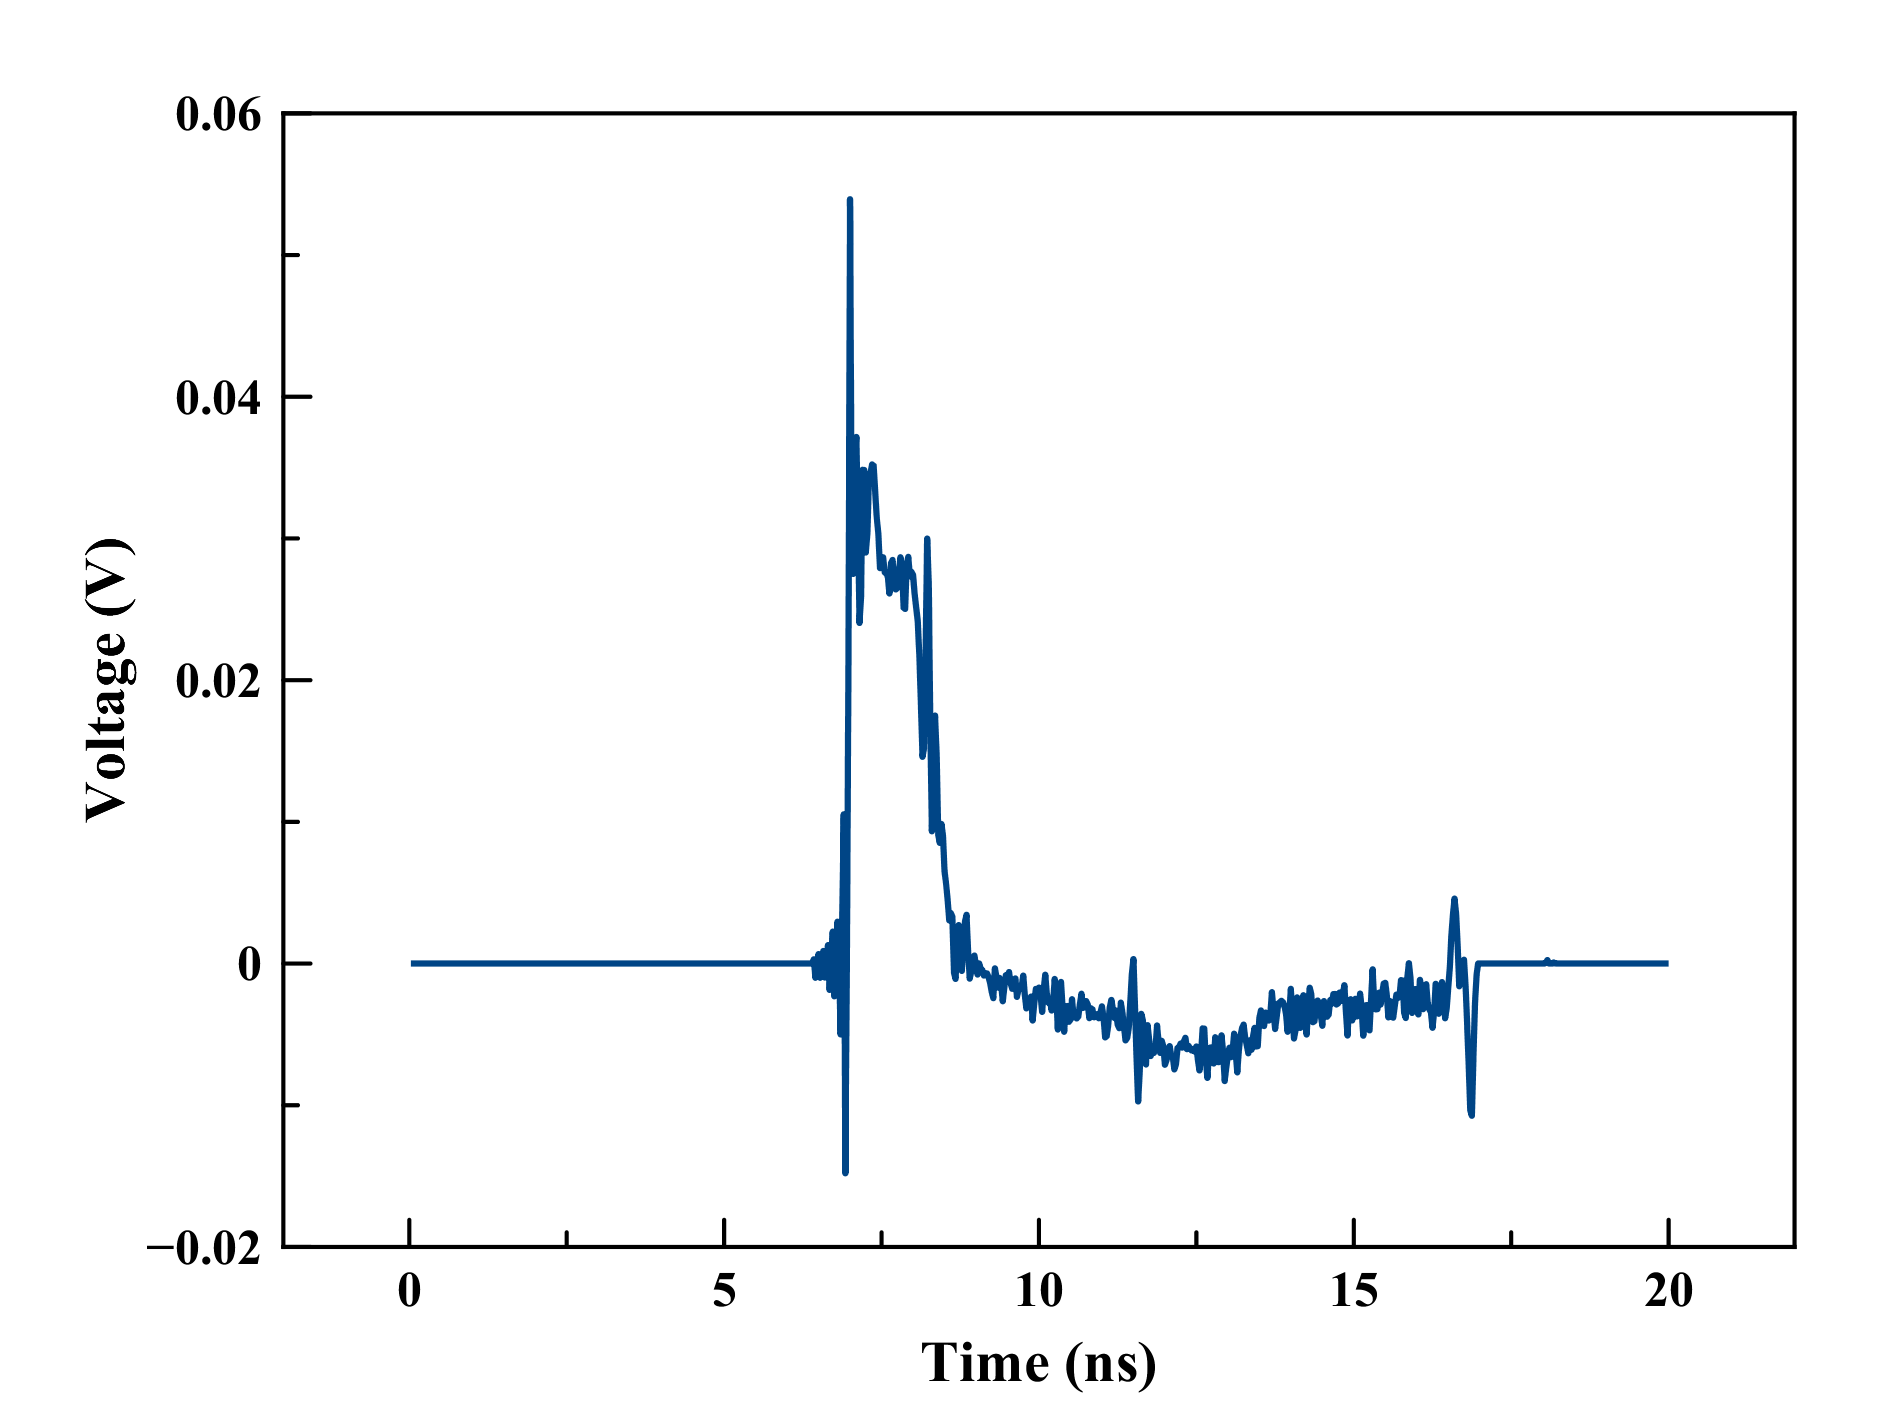
\includegraphics[width=80mm]{fig/2_6.png}}
\subfigure{\label{fig:67}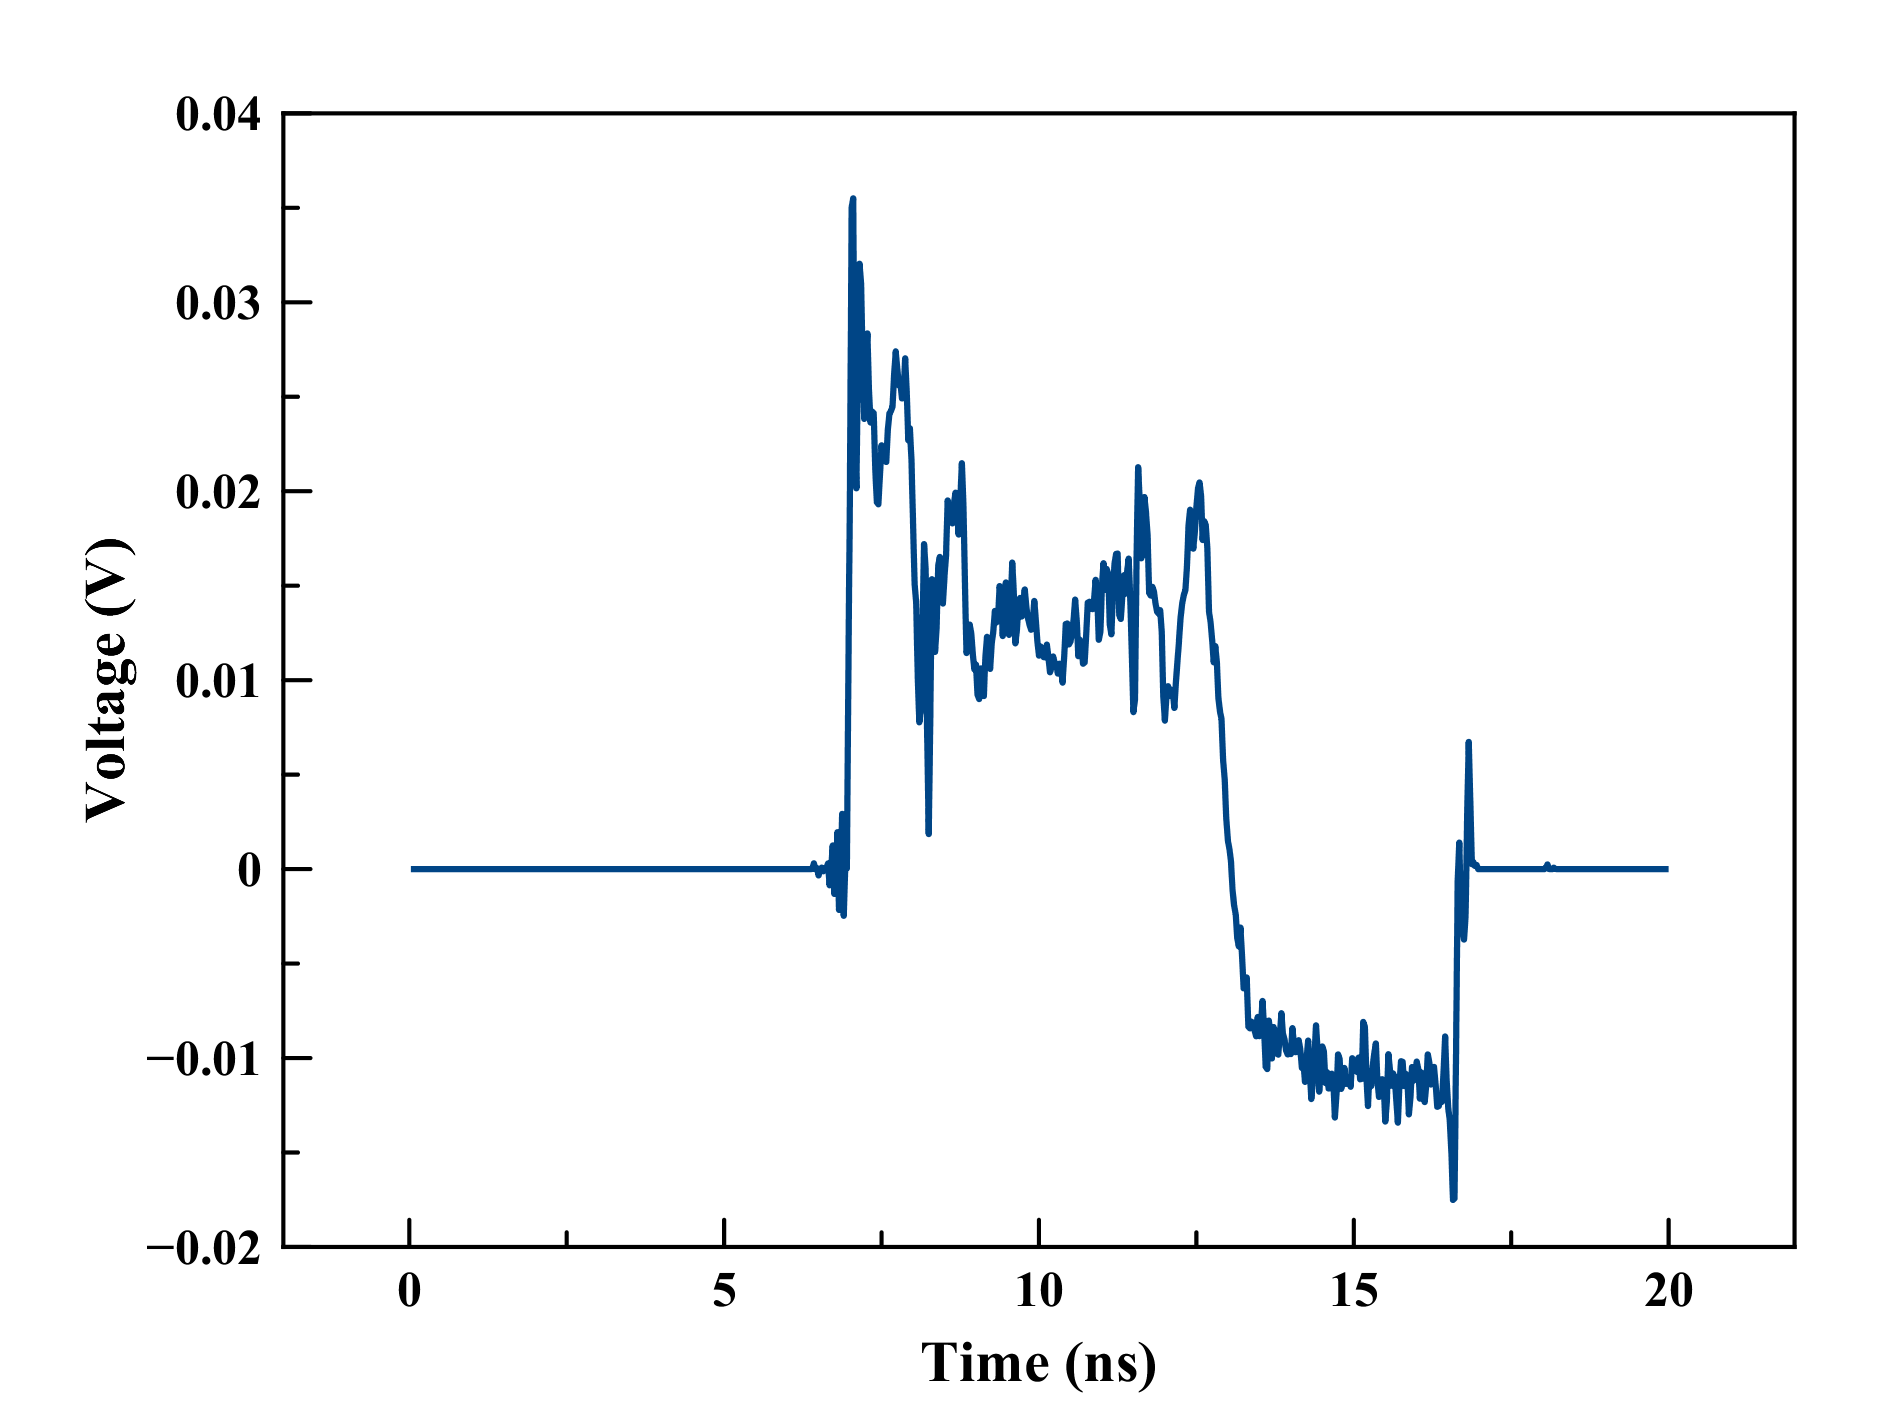
\includegraphics[width=80mm]{fig/6_7.png}}
\subfigure{\label{fig:9}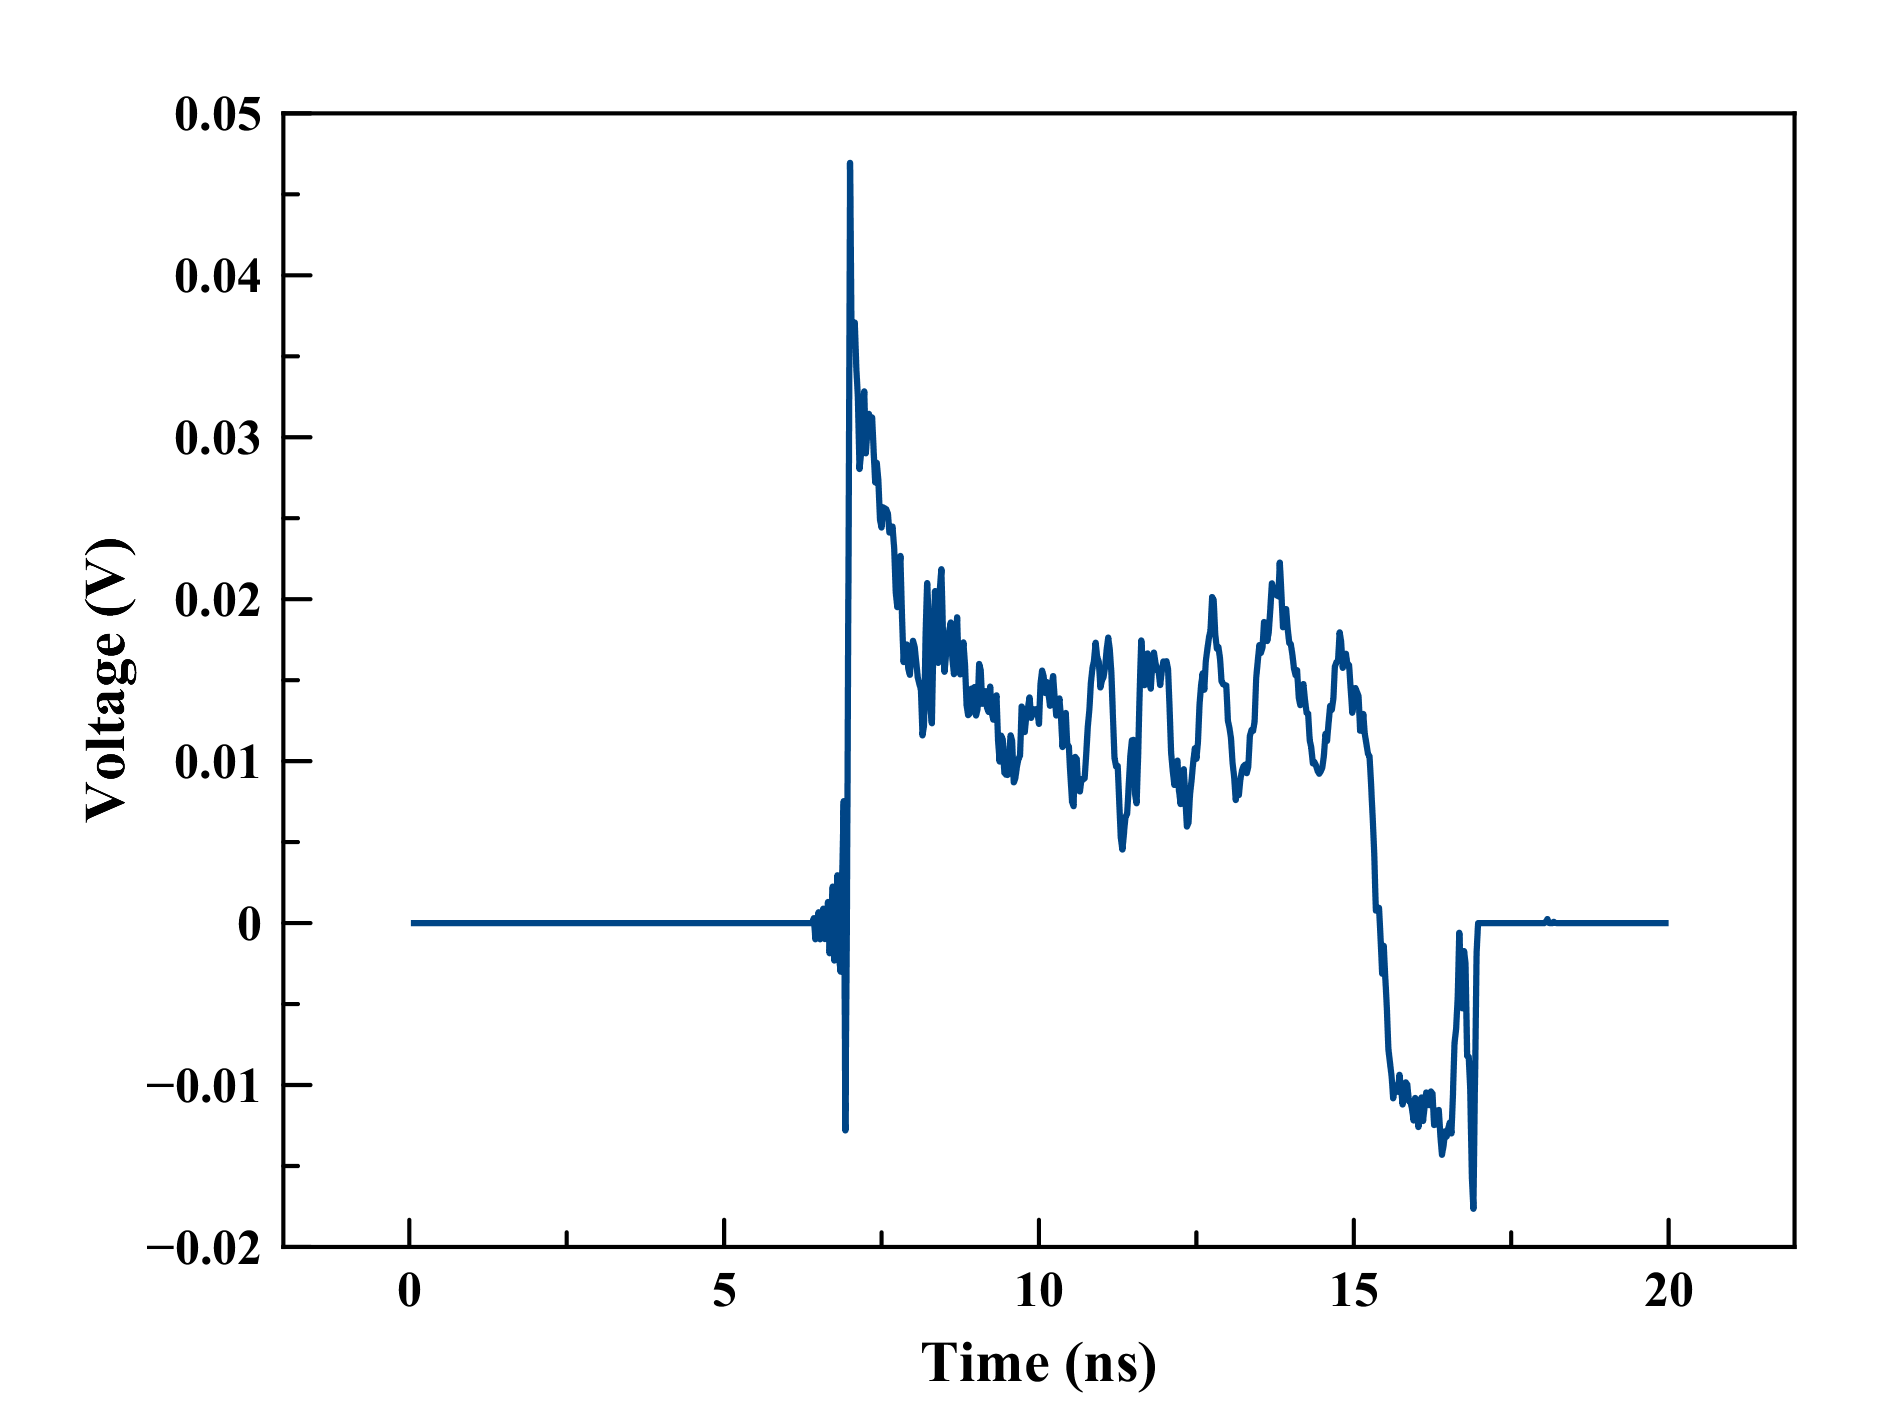
\includegraphics[width=80mm]{fig/9.png}}
\subfigure{\label{fig:no}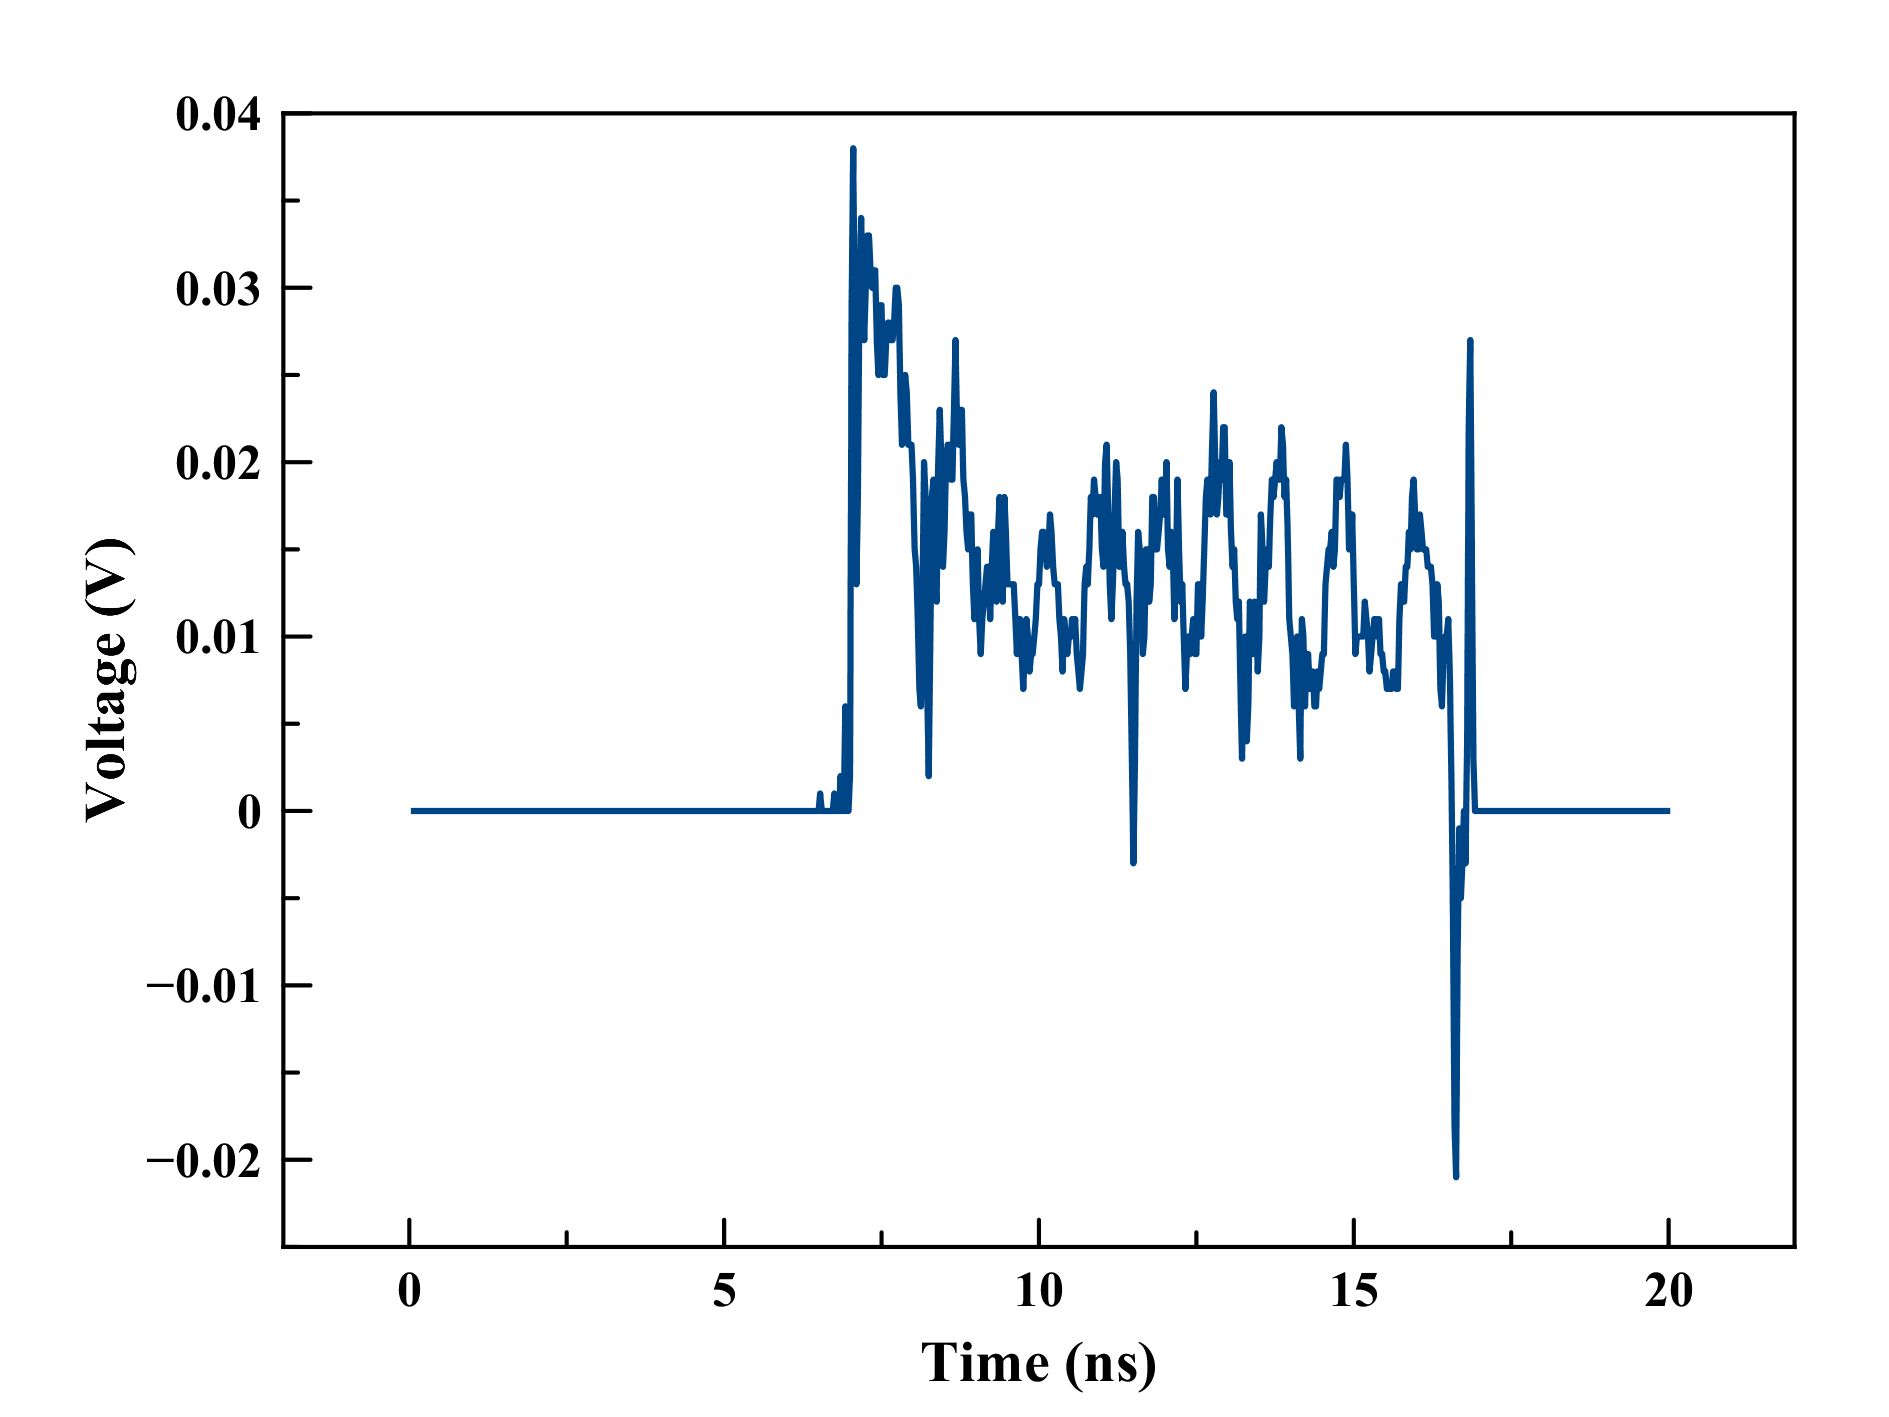
\includegraphics[width=80mm]{fig/no.png}}
\caption{Switching events for different individual events.(a)(b)(c) show switching events which switch at 2.6 ns, 6.7 ns and 9 ns respectively. (d) shows the non-switching event. }
\end{figure}

To further illustrate the random nature of magnetic switching in time-domain, we fix the applied voltage at 425 mV and study the distribution of the switching time as it is shown in Fig.\ref{fig:dist}. From other switching probability measurement, we already know that at 425 mV voltage, the device has a very switching probability. From this distribution we find that the switching time is unevenly distributed, it is centered around 4 ns and has a negative skewness. The distribution also gives a very small tail at high switching time, which means switching rarely happens at the tail of the pulse. We try to fit the switching count as a Gaussian function, which gives a good fitting result as it is shown in Fig.\ref{fig:dist}.



\begin{figure}[h]
  \centering
  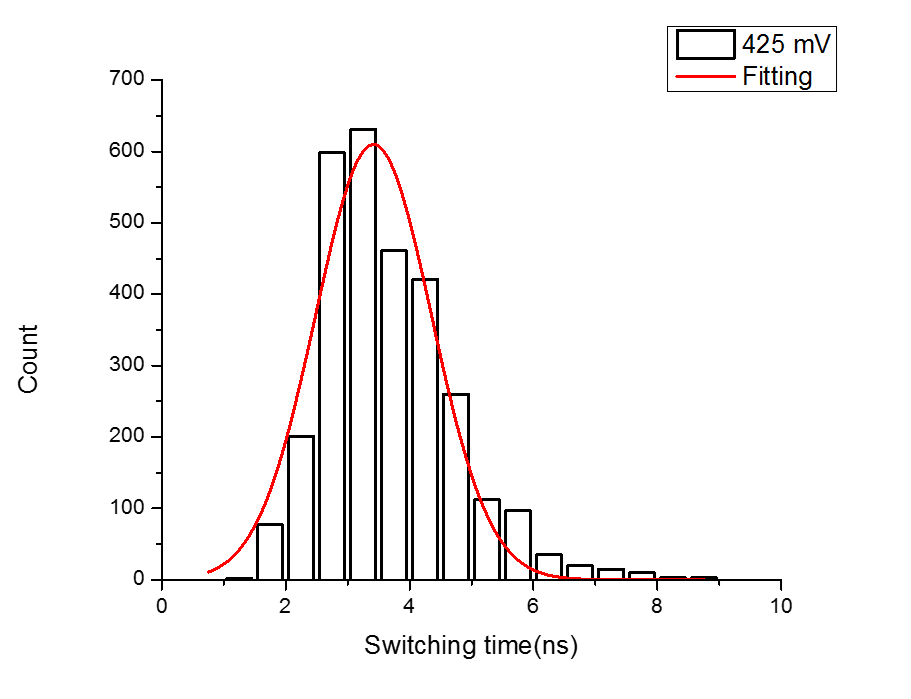
\includegraphics[width=0.8\textwidth]{fig/dist.png}
  \caption{Distribution of switching time at constant voltage 425 mV.}
  \label{fig:dist}
\end{figure}

If we vary the applied voltage and also measure the switching time distribution as Fig.\ref{fig:dist}, we typically find that the the peak of the distribution and also the skewness are dependent on the applied voltage. For smaller applied voltage, the center of the switching time moves to higher time period and the skewness of the distribution becomes smaller. That indicates that for larger voltage we have more deterministic and fast switching. When the applied voltage is small and the switching probability is low, the switching behavior shows more randomness.







